\documentclass[12pt]{article}

\usepackage[english]{babel}
\usepackage[utf8]{inputenc}
\usepackage{amsmath}
\usepackage{graphicx}
\usepackage[colorinlistoftodos]{todonotes}





\begin{document}




\section{Detector Operations}
The operation of the CMS detector continued relatively smoothly through to the end of the run. The LHC is now off for its annual Year End Technical Stop during which time maintenance will be performed on the accelerator and detectors. Since August the data tacking efficiency has consistently been greater than the 92.5\% taken last year. In early October a problem appeared in the pixel system that resulted is some loss of channels which is currently being investigated.   It is important to note that even with this issue the new pixel detector is now working better than the old one. 
\begin{figure}
\begin{center}
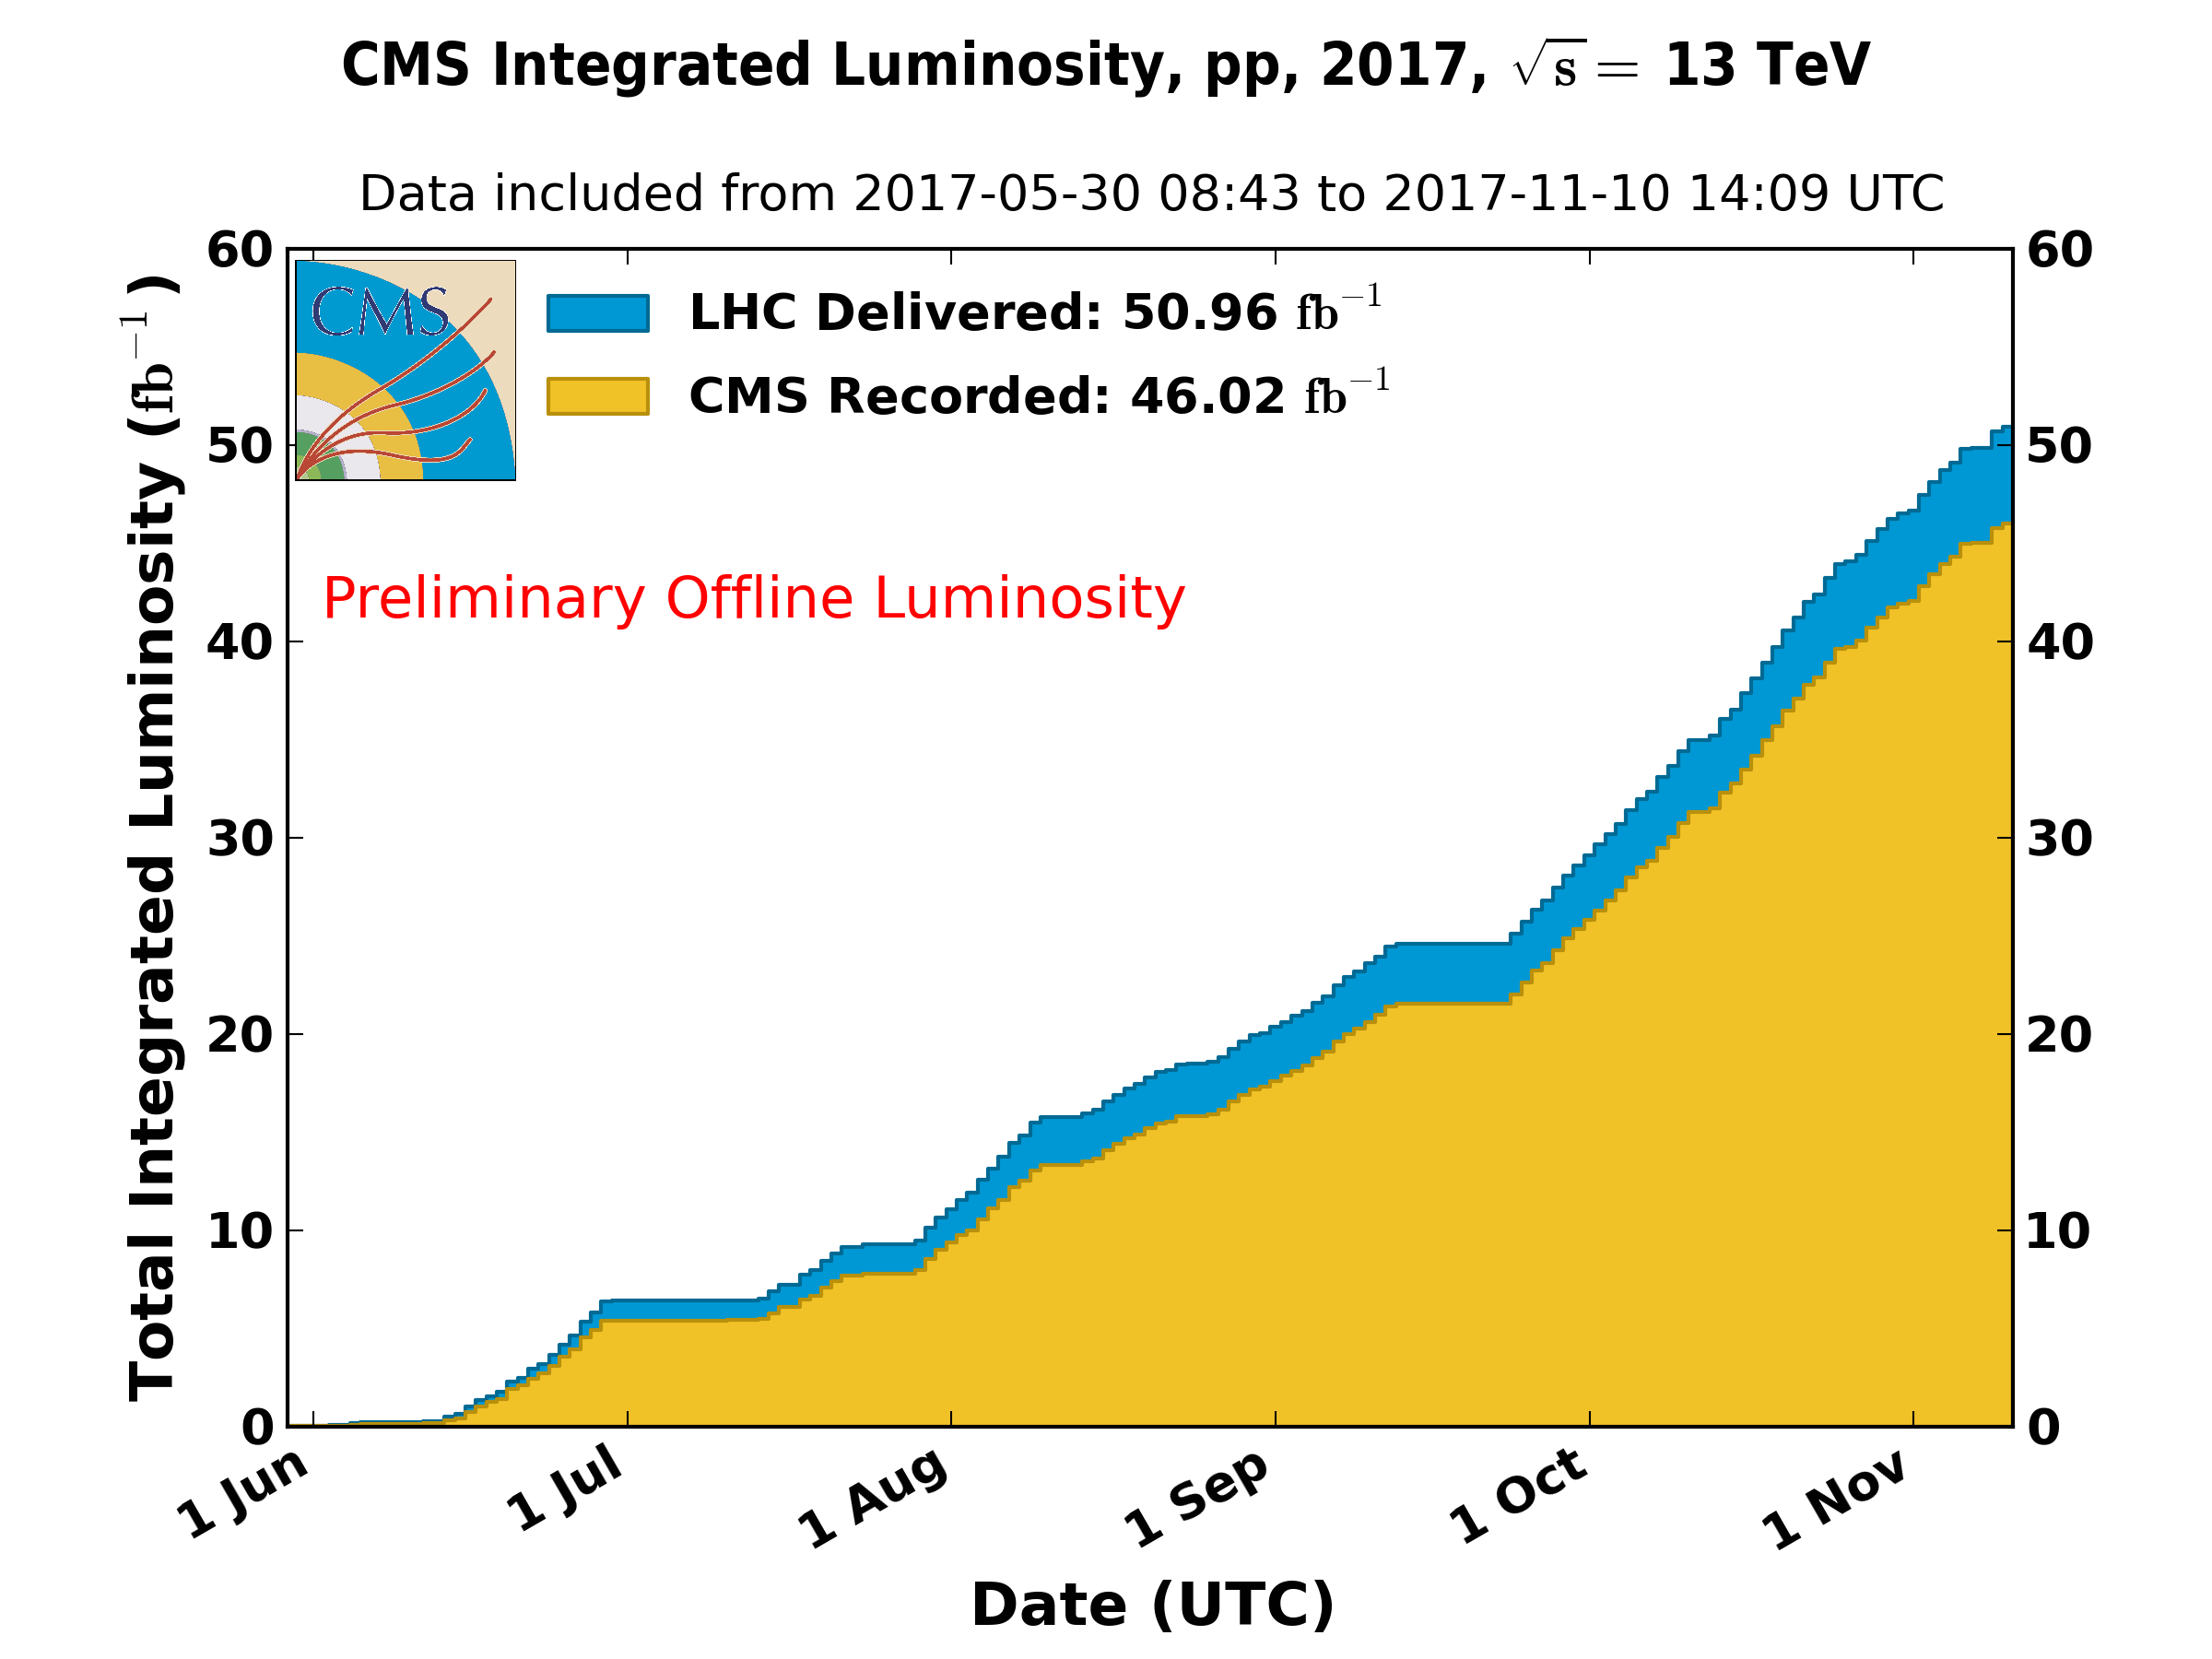
\includegraphics[width=0.66\textwidth]{int_lumi_per_day_cumulative_pp_2017NormtagLumi.png}
\caption{Luminosity, at 13 TeV, delivered by the LHC and recorded by CMS, in 2017.}
\label{fig:Lumi}
\end{center}
\end{figure}

\subsection{BRIL }

The Pixel Luminosity Telescope (PLT) together with the fast beam condition monitor (BCM1F) and HF provided online luminosity measurements continuously. The fast readout for all telescopes works but two telescopes exhibit degraded full pixel information that is used for track-based studies. Reconstructed tracks are also used for fast measurements of the beam spot and allow tracking of beam conditions. Corrections for efficiency and accidentals are obtained from analysis of tracks offline, and with fast turnaround after completion of each fill now. These corrections change with beam conditions and expected reduction of efficiency over time. Corrections are also obtained from mini-VdM scans at the start and end of a fill. Luminosity based on full track measurements was broadcast online. Systematic studies led to improved luminosity precision. Preliminary luminosity values have been obtained for the 2017 running (preapproval on 19 Dec).

The PLT must be extracted during the year end stop. The lab in P5 with two cold boxes was established and spare cards prepared in case of failures – the +z side was placed in the P5 lab on December 20 and its functionality tested. It is kept at $-10^o$~C. The –z side will be extracted in January.

\begin{table}[htp]
\caption{BRIL Metrics}
\begin{center}
\begin{tabular}{|l|r|}
\hline
Working Metric&Performance\\
\hline
Fraction of telescopes fully operational &  90\% \\
\hline
Efficiency of delivery of lumi histograms &  $>$ 99\% \\
\hline
Uptime of lumi  histogram production & $>$ 99\% \\
\hline
Lumi lost & 0 /pb \\
\hline
\end{tabular}
\end{center}
\label{BRILMetrics}
\end{table}%


\begin{table}[htp]
\caption{BRIL Milestones}
\begin{center}
\begin{tabular}{|l|l|r|r|}
\hline
Subsystem&Description&Scheduled&Achieved\\
\hline
BRIL & Update Lumi for 2016
& March 1& March 1\\
\hline
BRIL& Ready for Physics & May 1& May 1   \\
\hline
BRIL & Improve 2017 Lumi numbers & December  &  Preapp. Dec 19\\
\hline
\end{tabular}
\end{center}
\label{BRILMIlestones}
\end{table}%



\subsection{Tracker }

Operational concerns for the tracker were dominated by the 
loss of DCDC converters in the Pixel. Major downtimes were
noted for the strip cooling, some online timing and High 
Voltage scans and some strip FEDs getting stuck (sometimes
due to power issues). Major work was needed in the reconstruction
and simulation to keep up with the changing conditions in
the pixel detector. Data quality for this quarter was very
good as a result of the effort.

\subsubsection{Pixels }
\begin{figure}
\begin{center}
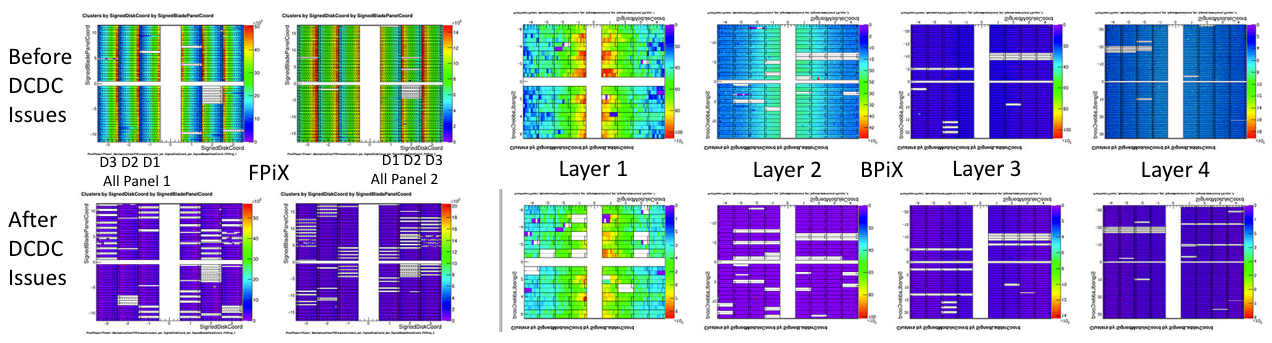
\includegraphics[width=0.95\textwidth]
{BeforeAndAfter.png}
\caption{The Pixel Detector cluster positions before DCDC converter issues appeared and at the end of running showing the loss of active channels due to non-functioning DCDC converters. New white areas indicate a loss of efficiency.}
\end{center}
\end{figure}
Starting October 5th, a number of pixel DCDC converters stopped delivering voltage to pixel modules. This occurred both in the Barrel (BPiX) and Forward (FPiX). DCDC converters became non-functional at power or enable/disable cycles. As a consequence, we shut off the automatic recovery for TBM single event upsets and instead did the recovery during inter-fill periods. In general, we lost about 0.5\% of the DCDC we cycled during recovery procedures or power cycles. In December, the FPiX detectors on the plus side of CMS were removed and the DCDC converters examined in detail. Preliminary results indicate an issue in one of the voltage regulators on the chip, though the root cause for the trouble is not proven. During the YETS, the rest of the pixel detector will be removed and new (or refurbished) DCDC converters will be installed prior to re-installation.  

\subsubsection{Strips}

The main issues in the strips are ongoing maintenance issues, such as power supply swaps, condition sensors etc. The Operations crew tries to minimize downtimes as these issue pop-up. The strips are looking to reduce time spent in SEU recovery and are recognizing the need for better long term solutions for maintaining the strip FEDs. The strips will be run colder in 2018 to allow more poorly cooled modules to have sufficient sensor voltage for physics.

\begin{table}[htp]
\caption{Tracker Metrics}
\begin{center}
\begin{tabular}{|l|c|c|}
\hline
 &Pixels&Strips\\
\hline
\% Working channels & 88.6 &  96.3 \\
\hline
Downtime attributed in pb$^{-1}$& 75.5 & 191.5 \\
Fraction of downtime attributed (\%)& 8.7 & 19.8\\
\hline
\end{tabular}
\end{center}
\label{TrackerMetrics}
\end{table}%


\begin{table}[htp]
\caption{Tracker Milestones}
\begin{center}
\begin{tabular}{|l|l|r|r|}
\hline
Subsystem&Description&Scheduled&Achieved\\
\hline
Tracker & Pixel Phase 0 Detector Removed&Feb 15&Jan 23 \\
\hline
Tracker & Pixel Phase 1 Detector Installed &Mar 30 &Mar 12 \\
\hline
Tracker & Pixel Phase 1 Detector & & \\ 
        & Ready for Collisions  &May 5 & Jun 16\\
\hline
\end{tabular}
\end{center}
\label{TrackerMilestones}
\end{table}%



\subsection{ECAL }
The ECAL continued to operate smoothly in the final three months of the run. There were no major incidents in any of the systems. Improvements in the DAQ efficiency came from better monitoring tools and consolidation of the single event upset (SEU) recovery procedures between ECAL and the ECAL pre-shower. Increase regularity of updating the laser corrections in the trigger improved the trigger turn on efficiency. The low voltage and laser systems operated without major problems. In December USCMS laser technician David Bailleux received a CMS detector award for “for outstanding contribution to all technical aspects of the ECAL and for his dedication to the ECAL laser system.”


\begin{table}[htp]
\caption{ECAL Metrics}
\begin{center}
\begin{tabular}{|l|r|}
\hline
Metric&Performance\\
\hline
Fraction of channels operational: EB& 99.1\% \\
\hline
Fraction of channels operational: EE& 98.4\%\\
\hline
Fraction of channels operational: ES& 99.9\%\\
\hline
Downtime attributed pb$^{-1}$ & 42 \\
Fraction of downtime attributed& 6\% \\
\hline
Resolution performance & 2.5\% \\
\hline
\end{tabular}
\end{center}
\label{ECALMetrics}
\end{table}%


\begin{table}[htp]
\caption{ECAL Milestones}
\begin{center}
\begin{tabular}{|l|l|r|r|}
\hline
Subsystem&Description&Scheduled&Achieved\\
\hline
ECAL & Refurbish Maraton to provide& &\\
     & redundant thermal interlock &March 1& March1 \\
\hline
ECAL & Replace Laser Diode & March 1& March 1\\
\hline
ECAL & Ready for Beam& May 1& May  1 \\
\hline
ECAL & Preliminary Calibration& June 15& July 15 \\
\hline
\end{tabular}
\end{center}
\label{ECALMilestones}
\end{table}%

\newpage

\subsection{HCAL}


\vspace{2mm}


During the fourth quarter of 2017, the HCAL Operations group focused continuing to take good data, and preparing
for the installation of the Phase 1 HE upgrades during the 2017-18 YETS.

The upgraded HF with dual anode readout and TDCs continued
to perform well. 
All the new handles to achieve noise reduction were in place earlier in the year and a substantial reduction
in missing Et trigger rates was been achieved. Energy recovery using the ``other'' anode when one anode
has an out-of-time signal was successfully implemented. The HE, with one upgraded HE readout box (out of 36) installed
to obtain experience with upgraded system, also continued to perform well.


During the quarter, HCAL downtime was only 1.7~pb$^{-1}$ out of more than 20~fb$^{-1}$ recorded.
For calendar 2017, HCAL downtime was 79~pb$^{-1}$ out of 45~fb$^{-1}$ recorded.




Planning to install the complete HE upgrade in 2017-18 YETS is complete. 
The plan enables installation even with the significant activity required
to remove and re-install the pixel detector.
The Installation Readiness Review for the HE Phase-1 upgrade during
YETS 17/18 was held November 6, and was successful. The items on the ``watch'' list from the review
have been completed. This includes 
the external low voltage for for the SiPM bias voltage replacing the DC-DC converters.

The observed damage in HE was confirmed to have a significant component from damage
to the HPDs as opposed to just scintillator damage.

A second HE readout box (HEP18) was installed in mid-December after the start of the YETS.
The installation went very smoothly. The time from being able to access the HE nose
to observing single PE peaks on all 192 channels after installation was less than 25 hours.

The final decision on installing the full upgrade will take place in January and has some
dependence on the pixel detector re-work.



Work on the HB Phase 1 upgrades, which will take place in LS2, also continued.
 
\vspace*{3mm}





\begin{table}[htp]
\caption{HCAL Metrics}
\begin{center}
\begin{tabular}{|l|r|}
\hline
Metric&Performance\\
\hline
Fraction of channels operational: HF& 100\%\ \\
\hline
Fraction of channels operational: HE& 99.85\%\ \\
\hline
Fraction of channels operational: HB& 99.77\% \\
\hline
Fraction of channels operational: HO& 99.72\%  \\
\hline
Downtime attributed pb$^{-1}$ & 78.9 \\
Fraction of CMS downtime due to HCAL& 3.1\%\ \\
\hline
Abs Energy Calibration & 2\% \\
\hline
Inter-calibration Uniformity & 2\% \\
\hline
\end{tabular}
\end{center}
\label{HCALMetrics}
\end{table}%



\begin{table}[htp]
\caption{HCAL Milestones}
\begin{center}
\begin{tabular}{|l|l|r|r|}
\hline
Subsystem&Description&Scheduled&Achieved\\
\hline
HCAL& HF Phase 1 Installed & April 1 &  March 15 \\
\hline
HCAL& HF Detector Commissioned & June 1 & May 1 \\
\hline
HCAL& Ready for Physics & June 1 & May 15\\
\hline
HCAL& Data Loss $<  1\%\ $  & July 15  & July 10\\
\hline
HCAL& 1\%\ to  2\%\  Calibration & July 15   &  Nov. 1 \\
\hline
\end{tabular}
\end{center}
\label{HCALMilestones}
\end{table}%












\subsection{EMU }

The CSC system completed the 2017 proton-proton run with 98.2\% of the 
channels active.  Many of the missing channels come from four chambers that 
were disabled at the beginning of 2017 data taking: two chambers 
(ME-1/1/34 and ME-1/1/35) without cooling due to water leaks, and  
two other chambers (ME-2/1/3 and ME-4/2/21) that are disabled due to low voltage problems. 
These will be investigated early in 2018 during the Year End Technical Stop (YETS).

The CSC detector shutdown started on Dec 4th. The gas system was stopped and chambers filled with backup gas mixtures (Ar 40\%, CO$_2$ 60\%). Two spare ME1/1 chambers are ready to be installed in place of ME-1/1/34 and/or ME-1/1/35 in case we would discover that the source of the cooling leak is coming from one of the on-chamber cooling circuit, though we believe this is unlikely. The two spares have been extensively tested in SX5 using our standard DAQ.

 During operations, there were several issues with the Maraton low voltage
supplies, with a total of six Maraton incidents in 2017.  Three of these were random self-switch-off events, and these are the main concern. Other users 
of these supplies are being consulted to try to learn if there is a systematic 
issue. The other faults were caused by CANbus communication issues. All will be investigated during YETS. 

During collisions, we observed a prominent excess in the local segment (trigger primitives) in the 
top region of the ME4/2 ring, where the rate was about three times higher than other 
regions in azimuth.  Studies with isolated bunches showed that these 
segments occurred two and three bunch crossings later than in-time muons.  These segments
 do not contribute to the L1 muon trigger rate because they do not correlate with other 
stations to form tracks, but they contribute to the DAQ occupancy.  It is being 
investigated if the source of this effect can be mitigated with additional shielding.  

Another excess was observed in the ME1/1 chambers during cosmic ray running in 
the hours following high luminosity runs.  These appear to be the result of 
activation of material near these chambers.  The rate from this source (about 250 Hz 
maximum) is negligible during collider operations. 

Both of these features and the results of these studies were reported to the CMS Technical Integration Group in November. 

The chamber gains continued to be studied after the HV changes were implemented to 
improve gain uniformity.  The goal is now to find a suitable operating point with 
lower gain to improve chamber longevity.  The plan is now to analyze the full 2017
data to reduce the gain uncertainties.  The milestone for implementing the reduced-gain
HV settings has been rescheduled for May 2019 in conjunction with the resumption of
collider operations. 

A productive mini workshop on CSC local reconstruction was held at CERN on Dec 12.  Several projects from many groups are ongoing towards developing improved algorithms and searching for new approaches in reconstruction of CSC hits and segments in order to maximize performance in high background and occupancy conditions, typical of high-luminosity running.  

A second round of exposure of muon electronics boards at CHARM II was completed in October, with 
a total dose of 37.2 kRad.  As expected, all the optical transmitters on the three
 DCFEBs in the test eventually failed by the time the exposure reached about 35 kRad.  The optical transmitters were then replaced on the irradiated boards, and subsequent tests showed the boards to be working properly otherwise.

 At the GIF++ facility, irradiation of the ME1/1 and mini-CSC with a mixture containing 2\% of CF$_4$ (instead of the usual 10\%) is in progress.  With an accumulated charge comparable to 1/3 HL-LHC  we observe no signs of aging so far. Parallel testing of a mini-CSC in B904 using a $^{90}$Sr source and 2\% CF$_4$ shows stable operation after the equivalent of one HL-LHC integrated charge.  This is of interest for possible future reduction in the use of 
CF$_4$, a potent greenhouse gas.



\begin{table}[htp]
\caption{CSC Metrics}
\begin{center}
\begin{tabular}{|l|c|}
\hline
 \% Working channels & 98.2\%  \\
\hline
Downtime attributed pb$^{-1}$ & 25.2 \\
Fraction of downtime attributed& 5\% \\
\hline
Median spatial resolution &  126 $\mu$m \\
\hline
\end{tabular}
\end{center}
\label{CSCMetrics}
\end{table}%



 \begin{table}[htp]
\caption{EMU Milestones}
\begin{center}
\def\arraystretch{1.5}

\begin{tabular}{|l|p{0.25\linewidth}|r|p{0.18\linewidth}|}
\hline
Subsystem&Description&Scheduled&Achieved\\
\hline
EMU& \raggedright{CSC ready for physics}& May 1& April 29 \\
\hline
EMU& \raggedright{Firmware to mitigate DCFEB EPROM problem} &July 1 &January 29\\ 
\hline
EMU & New HV settings for reduced gain &August 1 & Reschedule to May 2019 \\
\hline
\end{tabular}
\end{center}
\label{EMUMilestones}
\end{table}%


\subsection{DAQ}
The DAQ system continues to work without major issues. During the first few hours of luminosity leveling in each LHC fill, the DAQ handled 1.5\,MB events at 90\,kHz level-1 trigger rate and the HLT CPUs were up to 90\% loaded. The output of the HLT was typical 3\,GB/s. The pp-reference run stressed the storage and transfer system (SMTS) with a very high HLT output bandwidth of up to 6\,GB/s during a couple of days. Thanks to the close attention of the SMTS and tier-0 experts, no major problems occurred.

The only downtime caused by the DAQ system was due to circuit breakers tripping on a few racks containing filter-farm and builder-unit nodes. The investigation showed that 4 out of 24 racks had breakers with a too low current rating. A couple of filter-farm PCs were switched off in the affected racks to mitigate the problem. The circuit breakers were replaced after the end of the physics program.

The GEM detector has been integrated into the DAQ system. Provisions for the upgraded DT readout system ($\mu$ROS) and the new slink-express sender cards with an optical link developed for the ECAL readout have been made. Concerning the HLT, 400 Skylake-based machines have been ordered to replace the old C6220 nodes and the Huawei nodes on loan from CERN IT. The new machines will increase the HLT CPU capacity by 20\% compared to 2017. This should provide enough margin to cope with any LHC running condition in 2018 and mitigate any inefficiency from the pixel detector in case that the DCDC problem cannot be fixed during the YETS.

The DAQ monitoring tools were further improved. The most notable additions are the recording of the deadtime values together with the DAQ status information, and the improved diagnostic in the DAQ expert to pin-point the origin of the dead time. The addition of more case-based reasoning modules to the DAQ-expert, who proposed recovery procedures to the DAQ operator, have increased the overall DAQ running efficiency. 
Andre Holzner of UCSD received a CMS Detector Award ``For crucial contributions to many aspects of the CMS data acquisition, in particular the networking and monitoring for run-2.''

The development of the online monitoring system (OMS) is progressing. The second review held in December showed that more work is needed before the newly developed meta-data catalog can be deployed in production. The decision has been taken to postpone any further work on the final back-end system and to concentrate on deploying the new user interface as quickly as possible in 2018. The aim is to provide all required services with the new user interface, and to be able to retire the legacy WbM hardware and processes by end of 2018. The work on the back-end will resume once these goals have been achieved.


\begin{table}[htp]
\caption{DAQ Metrics}
\begin{center}
\begin{tabular}{|l|c|}
\hline
Dead time due to backpressure &0.65\%  \\
\hline
Downtime attributed pb$^{-1}$ &7.1 \\
Fraction of downtime attributed&0.07\% \\
\hline
\end{tabular}
\end{center}
\label{DAQMetrics}
\end{table}%
\begin{table}[h]
\caption{DAQ Milestones}
\begin{center}
\begin{tabular}{|l|l|r|r|}
\hline
Subsystem&Description&Scheduled&Achieved\\
\hline
DAQ& New sub-systems integrated  & Apr 1&Jun 15 \\
\hline
DAQ& Event builder expanded, & &\\
   & re-optimized for larger events & Jun 1 &Apr 1 \\
\hline
DAQ& Old HLT Nodes replaced & &\\
   & and new nodes commissioned & Jun 1 &Jun 21 \\
\hline
DAQ& Prototype of OMS (new WBM) & &\\ 
   & ready for field tests &Dec 31& \\
\hline
\end{tabular}
\end{center}
\label{DAQMilestones}
\end{table}%

\subsection{Trigger}

During this quarter the US groups continued their work on the Layer-1 calorimeter (CaloL1) trigger and the endcap muon trigger systems as both continued reliable data-taking. After completion of 2017 data-taking the groups worked on preparations for maintenance to be performed during the year-end shutdown.

\subsubsection{Endcap Muon Trigger}

The Northeastern, Rice University, and University of Florida groups
have maintained the EMTF system 24/7 during operations this quarter.  
A diagnosis of rare online control PC crashes exposed a clash of system
monitoring requests over PCIe. The EMTF firmware has been reworked and
successfully tested to improve arbitration. The SWATCH online
control software was updated with new reference values for EMTF registers. 

A study of an observed higher rate of LCTs (track stubs) originating
in ME4/2 at $\phi \approx 90^\circ$ has been
performed. Characteristics are consistent with beam or radiation
induced backgrounds. No significant impact on tracking performance is
observed. A study of the pile-up dependence of the muon trigger also
is ongoing, which shows that out-of-time segments do have an effect on
higher threshold muon triggers. Options to tighten the timing 
and spatial matching windows are under investigation. 

To debug occasional serial link errors between certain Muon Port Cards (MPCs)
and the EMTF, two versions of MPC firmware were loaded and the respective error
rates studied. The one with lower error rates (bypassing elastic buffers in
the FPGA) will be uploaded in 2018.

\subsubsection{Layer-1 Calorimeter Trigger}

The Layer-1 Calorimeter Trigger (CaloL1), built by the University of Wisconsin - Madison, is a part of the complete Calorimeter Phase-1 Trigger Upgrade. CaloL1 was in continuous operation during the LHC physics run in the last quarter of 2017.  Before cooling was shut down on December 6, the system was powered down for the Year-End Technical Stop (YETS) and currently remains off until cooling is restored and stable.

This was a relatively quiet quarter with a technical stop and two machine development periods.  CMS took p-p data at 13 and 5 TeV and participated in a short Xe-Xe reference run.  The only change to CaloL1 operations was to update the name to an alias for the uTCA bridge PC.  If a PC needs replacement this will make the operation transparent to CaloL1.

During this quarter, another of the ECAL links developed optical power issues.  This was resolved by simply moving the fiber on the ECAL side to the RCT position in the dual-transmitter VTTx. In addition, small discrepancies in the trigger primitives were observed in a couple of ECAL towers.  This became more pronounced near the end of the run, affecting multiple towers in ieta $\pm$20 and $\pm$26.  ECAL believed it was due to a timing alignment issue.

Final updates are under way to finish the work on the monitoring of the uTCA via the RCT DCS. During the YETS, the RCT WinCC OA was completely reinstalled to add a DIM framework and uTCA node to the finite state machine.  A DIM server that is accessed by the DIM framework is now running as a service on our CaloL1 SWATCH PC and is monitoring the uTCA by querying University of Wisconsin System Manager on our uTCA bridge PC.  This was done because it makes the bridge PC as generic as possible, the preference of the CMS Online System Administrators.
 
\begin{table}[htp]
\caption{Trigger Metrics}
\begin{center}
\begin{tabular}{|l|c|}
\hline
Frac of MPC Channels& 100\% \\
\hline
Frac of Upgrade EMUTF Channels& 100\% \\
\hline
Deadtime attributed to EMTF pb$^{-1}$ & 8.4 \\
Fraction of deadtime attributed to EMTF& 0.9\% \\
\hline
Frac of Calo. Layer-1 Channels & 100\% \\
\hline
Deadtime attributed to Calo. Layer-1 pb$^{-1}$ &  0\\
Fraction of deadtime attributed to Calo. Layer-1&  0\% \\
\hline
\end{tabular}
\end{center}
\label{TriggerMetrics}
\end{table}%
 
\begin{table}[h]
\caption{Trigger Milestones }
\begin{center}
\begin{tabular}{|l|l|r|r|}
\hline
Subsystem&Description&Scheduled&Achieved\\
\hline
TRIG&EMTF commissioned with & & \\
    & endcap RPC input &April 1 & April 27 \\
\hline
TRIG&EMTF ready for Physics &May 1& May 29\\
\hline
TRIG&Calo. Layer-1 commissioned &&\\
& with new ECAL/HCAL/HF Calib & April 1 & May 19\\
\hline
TRIG&Calo. Layer-1 Ready for physics&April  1&  May 19\\
\hline
\end{tabular}
\end{center}
\label{TriggerMilestones}
\end{table}%

\end{document}
